% Relatório de docking molecular — modelo LaTeX do agente AgRCK4MolDocking.
% Preencha General/Settings.tex e os capítulos; `agrck report ID` falha enquanto restar "PREENCHER".
% Compilação: pdflatex main && bibtex main && pdflatex main && pdflatex main
\documentclass[a4paper]{article}
% Useful packages, sorted so packages of similar functionality are grouped together. Not all are essential to make the document work, however an effort was made to make this list as minimalistic as possible. Feel free to add your own!

% Essential for making this template work are graphicx, float, tabularx, tabu, tocbibind, titlesec, fancyhdr, xcolor and tikz. 

% Not essential, but you will have to debug the document a little bit when removing them are amsmath, amsthm, amssymb, amsfonts, caption, subcaption, appendix, enumitem, hyperref and cleveref.

% inputenc, lipsum, booktabs, geometry and microtype are not required, but nice to have.

\usepackage[utf8]{inputenc} % Allows the use of some special characters
\usepackage[T1]{fontenc} % Proper font encoding for accented characters
\usepackage{amsmath, amsthm, amssymb, amsfonts} % Nicer mathematical typesetting
\usepackage{array} % Column types m{} and >{} in tables 

\usepackage{graphicx} % Allows the use of \begin{figure} and \includegraphics
\usepackage{float} % Useful for specifying the location of a figure ([H] for ex.)
\usepackage{caption} % Adds additional customization for (figure) captions
\usepackage{subcaption} % Needed to create sub-figures

\usepackage{tabularx} % Adds additional customization for tables
\usepackage{booktabs} % For generally nicer looking tables

\usepackage[nottoc,numbib]{tocbibind} % Automatically adds bibliography to ToC
\usepackage[margin = 2.5cm]{geometry} % Allows for custom (wider) margins
\usepackage{microtype} % Slightly loosens margin restrictions for nicer spacing  
\usepackage{titlesec} % Used to create custom section and subsection titles
\usepackage{titletoc} % Used to create a custom ToC
\usepackage{appendix} % Any chapter after \appendix is given a letter as index
\usepackage{fancyhdr} % Adds customization for headers and footers
\usepackage[shortlabels]{enumitem} % Adds additional customization for itemize. 

\usepackage{hyperref} % Allows links and makes references and the ToC clickable
\usepackage[noabbrev, capitalise]{cleveref} % Easier referencing using \cref{<label>} instead of \ref{}

\usepackage{xcolor} % Predefines additional colors and allows user defined colors

\usepackage{tikz} % Useful for drawing images, used for creating the frontpage
\usetikzlibrary{positioning} % Additional library for relative positioning 
\usetikzlibrary{calc} % Additional library for calculating within tikz

% Defines a command used by tikz to calculate some coordinates for the front-page
\makeatletter
\newcommand{\gettikzxy}[3]{%
  \tikz@scan@one@point\pgfutil@firstofone#1\relax
  \edef#2{\the\pgf@x}%
  \edef#3{\the\pgf@y}%
}
\makeatother




% ======================= DADOS DO RELATÓRIO (preencha) =======================
% Título do relatório
\newcommand\reporttitle{PREENCHER: Modelagem Molecular e Relação Estrutura--Atividade de <série> frente a <alvo>}

% Subtítulo (projeto, evento, disciplina...)
\newcommand\reportsubtitle{PREENCHER: Estudo teórico-computacional de suporte a <projeto>}

% Grupo / laboratório (aparece na capa)
\newcommand\groupnumber{\textbf{PREENCHER: Laboratório / Grupo --- Instituição}}

% Autores: "Nome & Vínculo \\" por linha
\newcommand\reportauthors{
PREENCHER: Nome do(a) autor(a) & Vínculo \\
}

% Instituição (linha abaixo da tabela de autores)
\newcommand\grouptutor{PREENCHER: Instituto --- Universidade}

% Local e data
\newcommand\placeanddate{PREENCHER: Cidade --- UF, Mês de Ano}

% Cabeçalho das páginas internas (esquerda e direita)
\newcommand\cabecalhoesq{PREENCHER: Grupo --- Instituição}
\newcommand\cabecalhodir{PREENCHER: título curto}

% Cor de destaque (títulos, marcadores, links)
\definecolor{corDestaque}{RGB}{0, 51, 102}
% ==============================================================================

% Sets up hyperlinks in the document to be colored
\hypersetup{
    colorlinks=true,
    linkcolor=corDestaque,
    urlcolor=corDestaque,
    citecolor = corDestaque
    }
\urlstyle{same}

% Portuguese names for ToC, Tables, Figures and Bibliography
\renewcommand{\contentsname}{Sumário}
\renewcommand{\figurename}{Figura}
\renewcommand{\tablename}{Tabela}
\renewcommand{\refname}{Referências Bibliográficas}
\crefname{figure}{Figura}{Figuras}
\Crefname{figure}{Figura}{Figuras}
\crefname{table}{Tabela}{Tabelas}
\Crefname{table}{Tabela}{Tabelas}
\crefname{section}{Seção}{Seções}
\Crefname{section}{Seção}{Seções}
\crefname{equation}{Equação}{Equações}
\Crefname{equation}{Equação}{Equações}

% Change bullet style for level 1, 2 and 3 respectively for itemize
\renewcommand{\labelitemi}{\scriptsize\textcolor{corDestaque}{$\blacksquare$}}% level 1
\renewcommand{\labelitemii}{\scriptsize\textcolor{corDestaque}{$\square$}}% level 2
\renewcommand{\labelitemiii}{\textcolor{corDestaque}{$\circ$}}% level 3

% Change bullet style for level 1, 2 and 3 respectively for enumerate
\renewcommand{\labelenumi}{\textbf{\textcolor{corDestaque}{\arabic*.}}}% level 1
\renewcommand{\labelenumii}{\textbf{\textcolor{corDestaque}{[\alph*]}}}% level 2
\renewcommand{\labelenumiii}{\textbf{\textcolor{corDestaque}{\roman*.}}}% level 3

% Have reference labels be linked to section
\counterwithin{equation}{section}
\counterwithin{figure}{section}
\counterwithin{table}{section}

% Creates header/footer
\pagestyle{fancy}
\lhead{\small\sffamily\textcolor{corDestaque}{\cabecalhoesq}}
\rhead{\small \cabecalhodir}
\renewcommand{\footrulewidth}{0.4pt}
\cfoot{Página \thepage}

% Formats section, subsection and subsubsection titles respectively
\titleformat{\section}{\sffamily\color{corDestaque}\Large\bfseries}{\thesection\enskip\color{gray}\textbar\enskip}{0cm}{}
\titleformat{\subsection}{\sffamily\color{corDestaque}\large\bfseries}{\thesubsection\enskip\color{gray}\textbar\enskip}{0cm}{}
\titleformat{\subsubsection}{\sffamily\color{corDestaque}\bfseries}{\thesubsubsection\enskip\color{gray}\textbar\enskip}{0cm}{}

% Formats captions
\DeclareCaptionFont{corDestaque}{\color{corDestaque}}
\captionsetup{labelfont={corDestaque,bf}, font=small}

% Changes font to mlmodern
\usepackage{mlmodern}

% Removes indent when starting a new paragraph
\setlength\parindent{0pt}
\setlength\parskip{5pt}

% Limits the ToC to sections and subsections
\setcounter{tocdepth}{2}

\begin{document}

% Capa
\begin{titlepage}

\centering

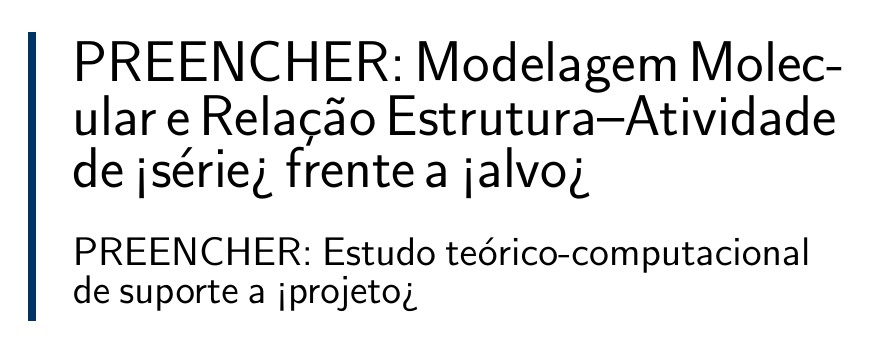
\begin{tikzpicture}

\node[text width = 0.8\textwidth](title){\sffamily\huge\reporttitle};

\node[text width = 0.8\textwidth, yshift = 0.75cm, below = of title](subtitle){\sffamily\Large \reportsubtitle};

\gettikzxy{(subtitle.south)}{\subtitlex}{\subtitley}
\gettikzxy{(title.north)}{\titlex}{\titley}
\draw[line width=1mm, corDestaque]($(title.west)+(-0.4,0)$) +(0,\subtitley) -- +(0,\titley);

\end{tikzpicture}
\vspace{2.5cm}

{\sffamily\groupnumber}

\begin{table}[H]
\centering
\sffamily
\large
\begin{tabularx}{0.85\linewidth}{lX}
\textbf{Pesquisador(a)} & \textbf{Vínculo}\\
\hline
\reportauthors
\end{tabularx}

\end{table}

{\sffamily \grouptutor}

\mbox{}
\vfill
{\color{corDestaque}\rule{\linewidth}{1mm}}\\[6pt]
\sffamily \Large \textcolor{corDestaque}{\placeanddate} \\

\end{titlepage}

\newpage

\pagenumbering{roman}

% Resumo
\section*{Resumo}
\addcontentsline{toc}{section}{Resumo}

\textbf{Contexto.} PREENCHER: origem da série (extrato, síntese), alvo terapêutico e dado experimental que motiva o estudo (ex.: \% de inibição ou $\text{IC}_{50}$ de cada composto).

\textbf{Objetivo.} PREENCHER: a pergunta central, em uma frase (ex.: que modo de ligação explica a atividade do composto líder frente aos análogos?).

\textbf{Metodologia.} PREENCHER: estruturas cristalográficas (código PDB), microespécies no pH do ensaio, amostragem por difusão (DiffDock-L), minimização local (GNINA), validação física (PoseBusters), seleção da pose no sítio ativo e mapeamento de interações (PROPKA3 + ProLIF).

\textbf{Resultados e discussão.} PREENCHER: RMSD do \textit{redocking}; métrica primária pré-registrada e as demais métricas; modo de ligação do líder e o que o distingue dos análogos; interações-chave atribuídas ao fragmento do ligante.

\textbf{Conclusões.} PREENCHER: hipóteses estruturais testáveis e as limitações do modelo (receptor rígido, ausência de águas explícitas, escores semiquantitativos, microespécie).

\vspace{6pt}
\textbf{Palavras-chave:} PREENCHER; \textit{docking} molecular; relação estrutura--atividade.

\newpage

% Sumário
{\hypersetup{linkcolor=black}
\tableofcontents\thispagestyle{empty}}
\newpage

% Lista de Símbolos, Siglas e Grandezas Físico-Químicas
\section*{Lista de Símbolos, Siglas e Grandezas Físico-Químicas} \label{section: symbols}

\begin{table}[H]
\centering
\caption{Siglas, sub-sítios e grandezas físico-químicas empregadas neste estudo.}
\vspace{4pt}
\small
\renewcommand{\arraystretch}{1.22}
\begin{tabularx}{\textwidth}{>{\bfseries}l X l}
\toprule
\textbf{Símbolo / Sigla} & \textbf{Conceito Bioquímico ou Físico-Químico} & \textbf{Unidade / Escala} \\
\midrule
PREENCHER & Alvo(s) e sub-sítios do receptor (ex.: sítio catalítico, sítio periférico, tríade catalítica), com os resíduos de cada um & --- \\
$\Delta G_{\text{Vina}}$ & Escore empírico de interação da função do AutoDock Vina (não é energia livre experimental) & $\text{kcal}\cdot\text{mol}^{-1}$ \\
$\text{CNN}_{\text{score}}$ & Probabilidade, estimada pela rede neural convolucional 3D do GNINA, de a pose estar a menos de $2,0\text{ \AA}$ da geometria nativa & $[0, 1]$ \\
$\text{CNN}_{\text{affinity}}$ & Afinidade predita pelo comitê de redes convolucionais 3D & $\text{p}K$ \\
$\text{LE}_{\text{Vina}}$ & Eficiência do Ligante: $-\Delta G_{\text{Vina}} / N_{\text{pesados}}$ & $\text{kcal}\cdot\text{mol}^{-1}\cdot\text{HA}^{-1}$ \\
$\text{RMSD}$ & Desvio quadrático médio dos átomos pesados entre a pose do \textit{redocking} e o cristal (corrigido por simetria) & $\text{\AA}$ (meta $\le 2,0\text{ \AA}$) \\
$d_{\text{sítio}}$ & Distância entre o centroide do ligante ancorado e o centroide do ligante cocristalizado & $\text{\AA}$ \\
$N_{\text{válidas}}/N$ & Fração das poses amostradas aprovada nas verificações físicas e estereoquímicas do PoseBusters & fração \\
$N_{\text{sítio}}/N$ & Poses fisicamente válidas que ocupam a cavidade ativa & fração \\
$\angle(\text{D--H}\cdots\text{A})$ & Ângulo doador--hidrogênio--aceitador de uma ligação de hidrogênio & graus ($^\circ$) \\
\bottomrule
\end{tabularx}
\end{table}

\newpage

% Seção 1: Introdução e Contextualização
\pagenumbering{arabic}
\section{Introdução e Contextualização} \label{section: introduction}

PREENCHER: contexto biológico do alvo e sua relevância terapêutica; anatomia do sítio de ligação (sub-sítios e resíduos, de preferência com uma figura didática); origem da série estudada e os dados experimentais que motivam a modelagem; a pergunta central do estudo.

As estruturas das moléculas discutidas ao longo do relatório estão reunidas na \cref{tab:estruturas}, que serve de guia para a leitura das seções seguintes.

\begin{table}[p]
\centering
\caption{Estruturas 2D das moléculas estudadas, geradas a partir dos SMILES usados no \textit{docking}. PREENCHER: modificação estrutural em relação ao composto líder e atividade medida.}
\label{tab:estruturas}
\renewcommand{\arraystretch}{1.1}
\begin{tabular}{>{\centering\arraybackslash}m{0.45\textwidth} >{\centering\arraybackslash}m{0.45\textwidth}}
PREENCHER: figura da pasta Figures/Estruturas \par (a) nome --- modificação --- atividade &
PREENCHER \par (b) nome --- modificação --- atividade \\
\end{tabular}
\end{table}

PREENCHER: tabela com os dados experimentais (atividade, concentração, controles do ensaio).

\newpage

% Seção 2: Protocolo de Modelagem Molecular
\section{Protocolo de Modelagem Molecular} \label{section: methodology}

\subsection{Fundamentação da Abordagem Híbrida de \textit{Docking}}

A predição do modo de ligação em cavidades profundas e confinadas precisa contornar duas limitações conhecidas \cite{Buttenschoen2024PoseBusters, McNutt2025GNINA13}:
\begin{itemize}
    \item \textbf{Amostragem limitada dos métodos clássicos em cavidades estreitas:} buscas estocásticas locais encontram dificuldade para transladar e rotacionar ligantes flexíveis através de constrições estreitas.
    \item \textbf{Geometria imperfeita de modelos generativos puros:} modelos de difusão equivariante no grupo $\text{SE}(3)$, como o \textit{DiffDock} \cite{Corso2023DiffDock, Corso2024DiffDockL}, exploram toda a proteína sem caixa de busca, mas podem gerar choques estéricos ou tensões torcionais, por não incluírem um termo explícito de repulsão de curto alcance \cite{Buttenschoen2024PoseBusters}.
\end{itemize}

Para combinar a busca global da difusão com o rigor dos campos de força, empregou-se um protocolo sequencial em seis etapas:

\begin{enumerate}
    \item \textbf{Seleção e preparo do receptor:} PREENCHER: estrutura cristalográfica (código PDB, resolução, ligante cocristalizado), cadeia retida e cofatores mantidos. O ligante cocristalizado define o centro do sítio ativo ($d_{\text{sítio}} = 0\text{ \AA}$) e serve de controle de \textit{redocking}. Glicanos de superfície e cossolventes de cristalização foram removidos.

    \item \textbf{Microespécies no pH do ensaio e geração conformacional:} os ligantes foram construídos com configuração absoluta definida em todos os estereocentros. O estado de protonação foi decidido pela equação de Henderson--Hasselbalch no pH do ensaio (PREENCHER):
    \begin{equation}
        \%\text{Protonada} = \frac{100}{1 + 10^{(\text{pH} - \text{p}K_a)}}
    \end{equation}
    Os confôrmeros iniciais foram gerados pelo algoritmo \texttt{ETKDGv3} \cite{Riniker2015ETKDG} e otimizados no campo de força \texttt{MMFF94}.

    \item \textbf{Amostragem global por difusão:} para cada ligante, PREENCHER poses independentes foram geradas pelo \textit{DiffDock-L} \cite{Corso2023DiffDock, Corso2024DiffDockL}, com restauração posterior da topologia química (ordens de ligação, cargas formais e hidrogênios explícitos).

    \item \textbf{Minimização local e validação física:} cada pose foi minimizada no receptor rígido com o \texttt{GNINA 1.3} \cite{McNutt2021GNINA10, McNutt2025GNINA13} e auditada pela suíte \texttt{PoseBusters} \cite{Buttenschoen2024PoseBusters}, que verifica comprimentos e ângulos de ligação, planaridade, quiralidade, choques intramoleculares e distância mínima proteína--ligante.

    \item \textbf{Pontuação, eficiência do ligante e critério topológico:} as poses válidas foram avaliadas por $\text{CNN}_{\text{score}}$, $\text{CNN}_{\text{affinity}}$ e $\Delta G_{\text{Vina}}$. Como escores aditivos favorecem moléculas maiores, calculou-se a eficiência do ligante:
    \begin{equation}
        \text{LE}_{\text{Vina}} = \frac{-\Delta G_{\text{Vina}}}{N_{\text{pesados}}}
        \label{eq:le_vina}
    \end{equation}
    A pose representativa de cada ligante é a de maior $\text{CNN}_{\text{score}}$ entre as poses aprovadas no PoseBusters e situadas no sítio ativo ($d_{\text{sítio}} \le$ PREENCHER $\text{\AA}$). A métrica usada para comparar os ligantes (PREENCHER) foi definida antes da obtenção dos resultados, e todas as métricas são relatadas.

    \item \textbf{Protonação do receptor e mapeamento de interações:} o receptor foi protonado no pH do ensaio com \texttt{PDB2PQR}/\texttt{PROPKA3} \cite{Olsson2011PROPKA3, Jurrus2018PDB2PQR}, e as interações foram tipificadas pelo \texttt{ProLIF} \cite{Bouysset2021ProLIF} com critérios de distância e de ângulo (ligação de hidrogênio, empilhamento $\pi$, cátion--$\pi$, contatos hidrofóbicos). Cada interação é atribuída ao fragmento do ligante (anel, açúcar ou substituinte) pelos índices atômicos.
\end{enumerate}

PREENCHER: tabela de propriedades físico-químicas dos ligantes (carga no pH do ensaio, massa molar, $N_{\text{pesados}}$, cLogP, TPSA, doadores/aceitadores de H, ligações rotacionáveis); use resizebox na tabela se houver muitas colunas.

\newpage

% Seção 3: Resultados e Discussão
\section{Resultados e Discussão} \label{section: results}

\subsection{Validação do Protocolo por \textit{Redocking}}
PREENCHER: RMSD do ligante cocristalizado (meta $\le 2,0\text{ \AA}$) e, se pertinente, o efeito da protonação do controle. Figura sugerida: sobreposição cristal $\times$ pose.

\subsection{Escores e Eficiência do Ligante}
PREENCHER: tabela com todas as métricas lado a lado ($\Delta G_{\text{Vina}}$, $\text{CNN}_{\text{affinity}}$, $\text{CNN}_{\text{score}}$, $\text{LE}_{\text{Vina}}$, $d_{\text{sítio}}$, $N_{\text{válidas}}/N$). Indique a métrica pré-registrada, se a posição do composto líder muda conforme a métrica e se a amplitude dos escores é suficiente para discriminar a série.

\subsection{Modo de Ligação e Interações}
PREENCHER: posição de cada ligante na cavidade e interações tipificadas (resíduo, tipo, distância, ângulo e fragmento do ligante). Figuras sugeridas: diagrama 2D de interações e figura 3D do sítio.

\subsection{Relação Estrutura--Atividade}
PREENCHER: o que diferencia os compostos ativos dos menos ativos segundo o modelo, sempre como hipótese estrutural.

\newpage

% Seção 4: Conclusões, Limitações e Perspectivas
\section{Conclusões, Limitações e Perspectivas} \label{section: conclusions}

PREENCHER: síntese das hipóteses estruturais propostas pelo modelo e dos determinantes de atividade sugeridos.

\subsection{Hipóteses Testáveis}
PREENCHER: previsões que os ensaios podem verificar (ex.: tipo de inibição na cinética enzimática, análogos a sintetizar ou testar).

\subsection{Limitações do Modelo}
\begin{itemize}
    \item Receptor rígido: a flexibilidade de cadeias laterais e de alças não foi amostrada.
    \item Águas estruturais não incluídas explicitamente no \textit{docking}.
    \item Escores semiquantitativos, que não equivalem a energia livre ou constantes de inibição experimentais.
    \item Microespécies modeladas: PREENCHER (formas consideradas e grupos com $\text{p}K_a$ próximo ao pH do ensaio).
    \item PREENCHER: emendas ao pré-registro, se houver.
\end{itemize}

\subsection{Perspectivas}
PREENCHER: refinamento por dinâmica molecular e cálculo de energia livre (por exemplo, MM-GBSA) e novos ensaios.

\newpage

% Referências Bibliográficas
\bibliographystyle{plain}
\bibliography{General/References}

\end{document}
